\documentclass[12pt,reqno]{amsart}
\usepackage{./header, amssymb}

\hdr{Mathematical Statistics}{Chapter 2: Probability spaces}

\begin{document}

\bigskip

\prob Let $A$ and $B$ be two subsets of a set $S$. Let $C$ be the subset of $S$ consisting of elements that are in $A$ or $B$, but not both. Express $C$ in terms of $A$ and $B$ using only the basic set operations.

\bigskip
\textcolor{red}{We have
	\[
	C = (A\cup B) \smallsetminus (A\cap B).
	\]}
\bigskip
















\prob Draw Venn diagrams to illustrate \text{DeMorgan's law}, which states that, given two subsets $A$ and $B$ of a set $S$, that

	\[
	(A\cup B)^c = A^c \cap B^c.
	\]

\bigskip
\textcolor{red}{We'll draw the Venn diagram in class.}
\bigskip











\prob Identify appropriate sample spaces for each of the following scenarios.

\medskip
\begin{enumerate}
\item Rolling a die.
    
\medskip
\textcolor{red}{$S = \{1,2,3,4,5,6\}$}
\bigskip

\item Flipping a coin.
    
\medskip
\textcolor{red}{$S = \{H,T\}$, where $H$ and $T$ stand for ``heads'' and ``tails,'' respectively.}
\bigskip

\item Flipping a coin \textit{three} times.
    
\medskip
\textcolor{red}{$S = \{HHH, HHT, HTH, HTT, THH, THT, TTH, TTT \}$}
\bigskip

\item Flipping a coin until it lands heads.
    
\medskip
\textcolor{red}{$S = \{H, TH, TTH, TTTH, TTTTH, \ldots\}$}
\bigskip

\item Forecasting whether it will rain tomorrow.
    
\medskip
\textcolor{red}{$S = \{\text{rain}, \text{no rain}\}$}
\bigskip

\item Conducting an experiment to measure the speed of light.
    
\medskip
\textcolor{red}{$S = [0,\infty)$. Theoretically, any non-negative real number could be obtained.}
\end{enumerate}











\bigskip
\prob Describe some events in the following scenarios. Use the sample spaces that you identified in the previous problem.

\medskip
\begin{enumerate}
\item Rolling a die.
    
\bigskip
\textcolor{red}{The event that we roll an even number is the subset
	\[
	A = \{2, 4, 6\} \subset S.
	\]}
\bigskip

\item Flipping a coin.
    
\bigskip
\textcolor{red}{The only subsets of $S$ are
	\[
	\emptyset, \\{H\\}, \\{T\\}, S,
	\]
so there aren't really any interesting events besides the simple ones.}
\bigskip

\item Flipping a coin \textit{three} times.
    
\bigskip
\textcolor{red}{The event that we flip exactly two heads is the subset
	\[
	A = \{HHT, HTH, THH\}\subset S.
	\]}
\bigskip

\item Flipping a coin until it lands heads.
    
\bigskip
\textcolor{red}{The event that we flip an even number of tails before we see a head corresponds to the subset
	\[
	A = \{ H, TTH, TTTTH, TTTTTTH, \ldots\} \subset S.
	\]}
\bigskip

\item Forecasting whether it will rain tomorrow.
    
\bigskip
\textcolor{red}{The only subsets of $S$ are
	\[
	\emptyset, \\{\text{rain}\\}, \\{\text{no rain}\\}, S,
	\]
so, there aren't really any interesting events besides the simple ones.}
\bigskip

\item Conducting an experiment to measure the speed of light.
    
\bigskip
\textcolor{red}{The event that you measure a number between 600 and 1000 (inclusive) is the subset
	\[
	A = [600, 1000].
	\]}
\end{enumerate}











\bigskip
\prob Suppose that you choose at random one of the twelve months of the year.

\begin{enumerate}
\item Identify an appropriate sample space.
    
\bigskip
\textcolor{red}{The sample space is the set of all twelve months:
	\[
	S = \{\text{January}, \text{February},\ldots,\text{December}\}.
	\]}
\bigskip

\item Identify the event that you choose a month beginning with a ``J''.
    
\bigskip
\textcolor{red}{This is the event
	\[
	A = \{\text{January}, \text{June}, \text{July} \}.
	\]}
\bigskip

\item Identify the event that you choose a month whose name is four letters long.
    
\bigskip
\textcolor{red}{This is the event
	\[
	B = \{\text{June},\text{July} \}.
	\]}
\bigskip

\item Using one of the basic set operations and your answers to the two previous parts, identify the event that you choose a month beginning with a ``J'' and whose name is four letters long.
    
\bigskip
\textcolor{red}{This is the event
	\[
	A\cap B= \{\text{June}\}.
	\]}
\end{enumerate}
























\bigskip
\prob Suppose that $A$ and $B$ are two events. Write expressions involving only the basic set operations for each of the following:

\bigskip
\begin{enumerate}
\item Both events occur. \textcolor{red}{$A\cap B$}
\item At least one occurs. \textcolor{red}{$A\cup B$}
\item Neither occurs. \textcolor{red}{$S \smallsetminus (A\cup B)$}
\item Exactly one occurs. \textcolor{red}{$(A\cup B)\smallsetminus(A\cap B)$}
\end{enumerate}








\bigskip
\prob Let $P$ be the discrete probability measure on the sample space $S=\mathbb{R}$ with probability mass function

	\[
	p(s) = \begin{cases}
	1/4 & : s=0, \\
	1/4 & : s=2, \\
	1/2 & : s=4, \\
	0 & : \text{otherwise}.
	\end{cases}
	\]

Compute the probabilities $P(A)$ of the following events.

\medskip
\begin{enumerate}
\item $A = [-2, -1]$
    
\bigskip
\textcolor{red}{We have
	\[
	P(A) = 0,
	\]
since $A$ does not contain $s=0$, $2$, or $4$.}
\bigskip

\item $A = (-1, 1)$
    
\bigskip
\textcolor{red}{We have
	\[
	P(A) = 1/4,
	\]
	since $A$ contains $s=0$.}
\bigskip

\item $A = (-1, 1) \cup (3,5]$
    
\bigskip
\textcolor{red}{We have
	\[
	P(A) = 1/4 + 1/2 = 3/4,
	\]
since $A$ contains $s=0$ and $4$.}
\bigskip
    
\item $A = \mathbb{R}$
    
\bigskip
\textcolor{red}{We have
	\[
	P(A) = 1/4 +1/4+ 1/2 = 1,
	\]
since $A$ contains $s=0$, $2$, and $4$.}
\end{enumerate}









\bigskip
\prob Let $P$ be the discrete probability measure on the sample space $S=\mathbb{R}$ with probability mass function

	\[
	p(s) = \begin{cases}
	(0.25) (0.75)^{s-1} & : s=1, 2, 3, \ldots, \\
	0 & : \text{otherwise}.
	\end{cases}
	\]

Compute the probabilities $P(A)$ of the following events.

\medskip
\begin{enumerate}
\item $A = (-\infty,1)$
    
\bigskip
\textcolor{red}{We have
	\[
	P(A) = 0,
	\]
since $A$ does not contain any positive integer.}
\bigskip

\item $A = (-10, 4]$
    
\bigskip
\textcolor{red}{We have
	\[
	P(A) = 0.25 + (0.25)(0.75) + (0.25)(0.75)^2+ (0.25)(0.75)^3\approx 0.68,
	\]
since $A$ contains $n=1,2,3,4$.}
\bigskip

\item $A = \mathbb{R}$
    
\bigskip
\textcolor{red}{We have
        \[
        P(A) = \sum_{s=1}^\infty (0.25)(0.75)^{s-1} = \frac{0.25}{1-0.75} = 1,
        \]
    since $A$ contains all positive integers.}
\bigskip
    
\item $A = \{\text{all positive even integers}\}$
    
\bigskip
\textcolor{red}{We have
	\[
	P(A) = \sum_{s=1}^\infty (0.25)(0.75)^{2s-1} = \frac{0.25}{0.75} \cdot \frac{(0.75)^2}{1-(0.75)^2} \approx 0.43.
	\]}
\end{enumerate}
















\bigskip
\prob Describe in complete detail a probability space that models each of the following scenarios. Be sure to check that the two requirements in the Discrete Probability Construction Lemma are both satisfied.

\medskip
\begin{enumerate}
\item Rolling a fair six-sided die.

\bigskip
\textcolor{red}{Remember, there are three things that go into a probability space: The sample space, the collection of events, and the probability measure. For this problem, the sample space is
	\[
	S = \{ 1, 2, 3, 4, 5, 6\}
	\]
where each integer $s\in S$ represents an outcome of rolling the die. The collection of events will be \textit{all} subsets. The probability measure $P$ is uniform with probability function given by
	\[
	p(s) = 1/6,
	\]
for each $s\in S$. Since these probabilities sum to $1$ over all six sample points, the Construction Lemma guarantees that we have a valid probability measure.}
\bigskip

\item Flipping an \textbf{unfair} coin, with probability $0.25$ of obtaining heads, and probability $0.75$ of obtaining tails.
    
\bigskip
\textcolor{red}{The probability space has sample space
	\[
	S = \{H,T\}
	\]
where $H$ represents the outcome of obtaining heads and $T$ the outcome of obtaining tails. The collection of events is \textit{all} subsets. The probability measure is discrete with probability function given by
	\[
	p(H) = 0.25 \quad \text{and} \quad p(T) = 0.75.
	\]
Since $0.25+0.75=1$, the Construction Lemma guarantees that we have a valid probability measure.}
\bigskip

\item Flipping an \textbf{unfair} coin twice, with probability $0.25$ of obtaining heads, and probability $0.75$ of obtaining tails. What is the probability that you flip \textit{exactly} one head?
    
\bigskip
\textcolor{red}{The probability space has sample space
	\[
	S = \{HH,HT, TH, TT\}
	\]
where $H$ represents the outcome of obtaining heads and $T$ the outcome of obtaining tails. The collection of events is \textit{all} subsets. The probability measure is discrete with probability function given by
	\[
	p(HH) = (0.25)^2 \quad p(HT) = (0.25)(0.75), \quad p(TH)= (0.25)(0.75), \quad p(TT) = (0.75)^2 .
	\]
Since
	\[
	(0.25)^2 + (0.25)(0.75) + (0.25)(0.75) + (0.75)^2 = 1,
	\]
the Construction Lemma guarantees that we have a valid probability measure. The probability that we flip \textit{exactly} one head is
	\[
	P(\{HT,TH\}) = p(HT) + p(TH) = 2(0.25)(0.75) = 0.375.
	\]}
\bigskip

\item Flipping an \textbf{unfair} fair coin until you obtain a head, with probability $0.25$ of obtaining heads, and probability $0.75$ of obtaining tails. What is the probability that you flip an odd number of tails before you see a head?
    
\bigskip
\textcolor{red}{The probability space has sample space
	\[
	S = \{ H, TH, TTH, TTTH, \ldots\}.
	\]
The collection of events is \textit{all} subsets. The probability measure is discrete with probability function given by
	\[
	p(\underbrace{T\cdots TH}_{\text{$n$ flips}}) = (0.25)(0.75)^{n-1}.
	\]
But is this \textit{really} a valid probability measure? If you remember your rules for infinite series from calculus, you'll notice that:
	\[
	\sum_{n=1}^\infty (0.25)(0.75)^{n-1} = \frac{0.25}{1-0.75} = 1,
	\]
so indeed the Construction Lemma guarantees that we obtain a valid probability measure. The probability that we flip an odd number of tails before we see a head is
	\[
	\sum_{n=1}^\infty (0.25)(0.75)^{2n-1} = \frac{0.25}{0.75} \cdot \frac{(0.75)^2}{1-(0.75)^2} \approx 0.43.
	\]}
\end{enumerate}

















\bigskip
\prob A sample space consists of five simple events, $E_1$, $E_2$, $E_3$, $E_4$, and $E_5$.

\medskip
\begin{enumerate}
\item If $P(E_1) = P(E_2) = 0.15$, $P(E_3) = 0.4$, and $P(E_4) = 2P(E_5)$, find the probabilities of $E_4$ and $E_5$.
    
\bigskip
\textcolor{red}{We know that the total probability must sum to $1$, so
	\[
	1 = \sum_{i=1}^5P(E_i) = 0.15 + 0.15 + 0.4 + P(E_4) + 2P(E_4).
	\]
Solving this equation for $P(E_4)$ gives $0.1$, from which it follows that $P(E_5)=0.2$.}
\bigskip

\item If $P(E_1) = 3P(E_2) = 0.3$, find the probabilities of the remaining simple events if you know that the remaining simple events are equally probable.
    
\bigskip
\textcolor{red}{Same strategy as the first part. We know that
	\[
	1 = \sum_{i=1}^5P(E_i) = 0.3 + 0.3/3 + P(E_3) + P(E_3) + P(E_3),
	\]
and solving this for $P(E_3)$ yields $0.2$. But then this must also be the probability $P(E_4)$ and $P(E_5)$, as well.}
    
\end{enumerate}















\bigskip
\prob A survey classified a large number of adults according to whether they were diagnosed as needing eyeglasses to correct their reading vision and whether they use eyeglasses when reading. The proportions falling into the four resulting categories are given in the following table:

\medskip
\begin{center}
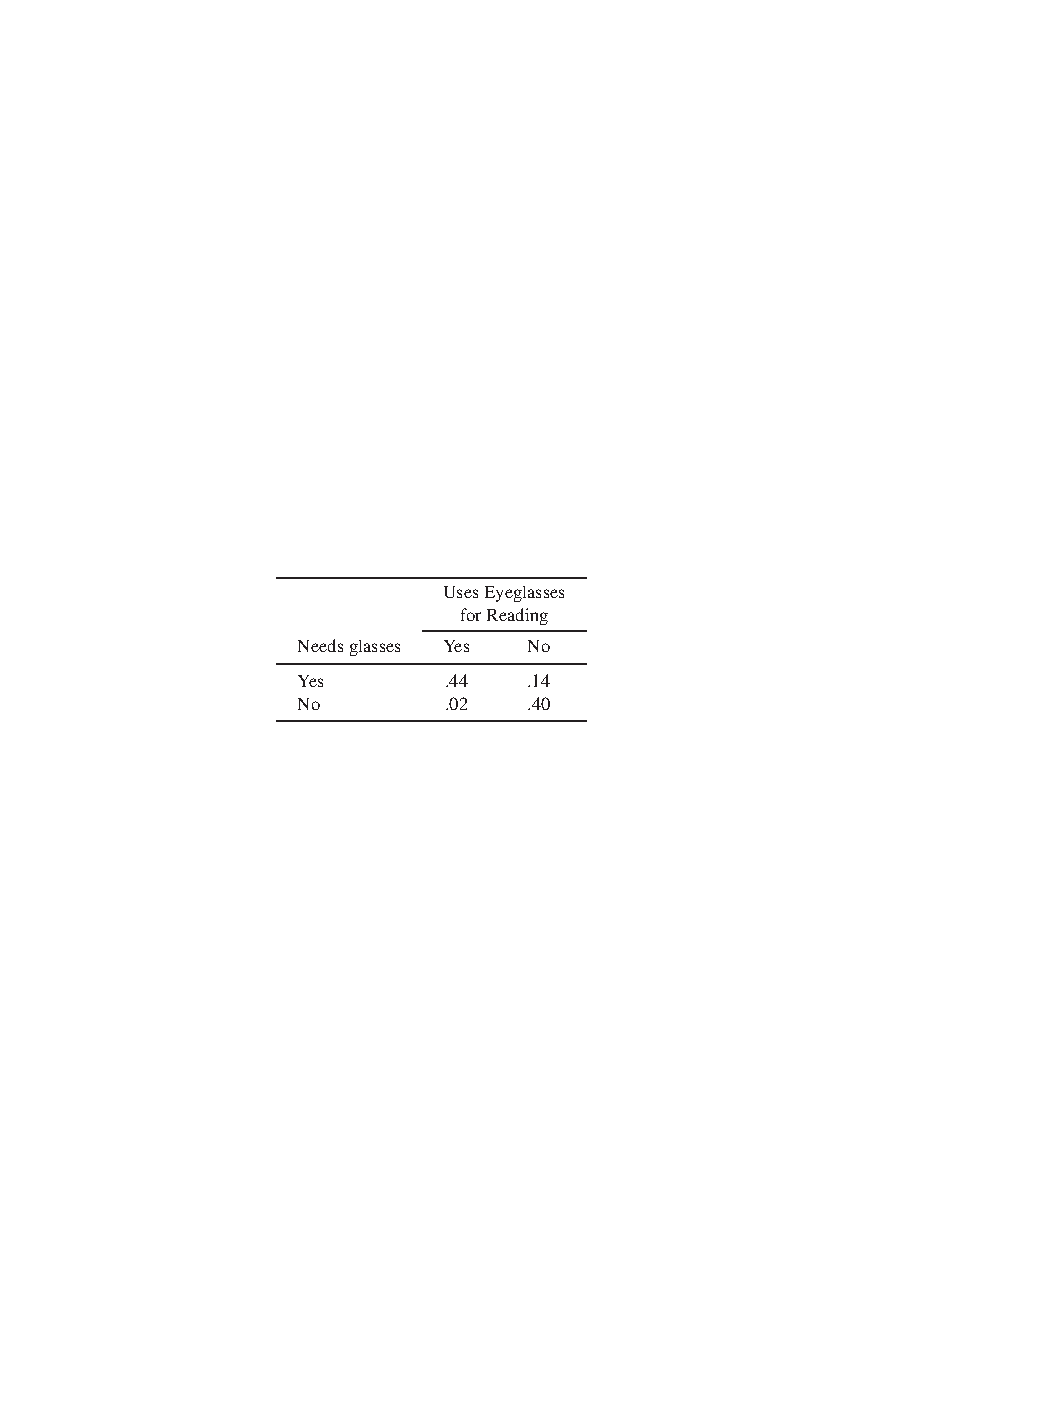
\includegraphics[scale=1]{img.pdf}
\end{center}
\medskip

If a single adult is selected from the large group, find the probabilities of the events defined below. The adult

\medskip
\begin{enumerate}
\item needs glasses.
    
\bigskip
\textcolor{red}{Since the adult is selected at random, any one adult has the same chance as being selected as any other. Therefore, the proportions listed in the table \textit{are} the probabilities that a randomly chosen adult falls into one of the four groups in the table. Therefore, for part (a), the probability is $0.44 + 0.14 = 0.58$, which is the sum of the probabilities of the two groups that both need glasses.}
\bigskip

\item needs glasses but does not use them.
    
\bigskip
\textcolor{red}{$0.14$}
\bigskip

\item uses glasses whether the glasses are needed or not.
    
\bigskip
\textcolor{red}{$0.44+0.02=0.46$}
\bigskip
\end{enumerate}














\bigskip
\prob Let $P$ be a continuous probability measure on the sample space $S=\mathbb{R}$ with probability density function

	\[
	f(s) = \begin{cases}
	\frac{2}{9}s & : 0 \leq s \leq 3, \\\
	0 & : \text{otherwise}.    
	\end{cases}
	\]

Compute the probabilities $P(A)$ of the following events.

\medskip
\begin{enumerate}
\item $A=(-1, 1]$
    
\bigskip
\textcolor{red}{We have:
	\[
	P(A) = \int_{-1}^1 f(s) \ \text{d}s = \frac{2}{9}\int_0^1 s \ \text{d} s = \frac{1}{9}.
	\]}
\bigskip

\item $A = (-1,1) \cup [2, 4)$.
    
\bigskip
\textcolor{red}{We have:
	\[
	P(A) = \int_{-1}^1f(s) \ \text{d}s + \int_2^4 f(s) \ \text{d}s = \frac{2}{9} \int_0^1 s \ \text{d}s + \frac{2}{9} \int_2^3 s \ \text{d}s = \frac{2}{3}.
	\]}
\bigskip

\item $A = [0,3]$.
    
\bigskip
\textcolor{red}{We have:
	\[
	P(A) = \int_{0}^3f(s) \ \text{d}s = \frac{2}{9} \int_0^3 s \ \text{d}s =1.
	\]}
\bigskip

\item $A = \mathbb{R}$.
    
\bigskip
\textcolor{red}{We have:
	\[
	P(A) = \int_{-\infty}^\infty f(s) \ \text{d}s = \frac{2}{9} \int_0^3 s \ \text{d}s =1.
	\]}
\end{enumerate}











\bigskip
\prob Let $P$ be a continuous probability measure on the sample space $S=\mathbb{R}$ with probability density function

	\[
	f(s) = \begin{cases}
	\displaystyle\frac{1}{s^2} & : s \geq 1, \\\
	0 & : \text{otherwise}.    
	\end{cases}
	\]

Compute the probabilities $P(A)$ of the following events.

\medskip
\begin{enumerate}
\item $A=(-10, 0)$
    
\bigskip
\textcolor{red}{We have:
	\[
	P(A) = \int_{-10}^0 f(s) \ \text{d}s = 0.
	\]}
\bigskip

\item $A = \mathbb{R}$.
    
\bigskip
\textcolor{red}{We have:
	\[
	P(A) = \int_{-\infty}^\infty f(s) \ \text{d}s = \int_1^\infty \frac{1}{s^2} \ \text{d}s = \left(\lim_{s\to \infty} \frac{1}{s}\right) + 1 = 1.
	\]}
\end{enumerate}








\bigskip
\prob A particle is located somewhere along the real line $\mathbb{R}$, but the \text{only} information that you have about its location is that it is at some point in the interval $[0,4]$.

\medskip
\begin{enumerate}
\item Describe in complete detail a probability space that models this scenario.

\bigskip
\textcolor{red}{This scenario may be modeled by a continuous probability distribution $P$. We may define $P$ by using the Continuous Probability Construction Lemma by defining its probability density function. Since we know that the particle can only be in the interval $[0,4]$, we set $f(s)=0$ for all $s$ outside this interval. In the absence of any more information about its location in $[0,4]$, it makes sense to assume that the density function $f(y)$ is uniform (i.e., constant) across this interval. (This is called a \textit{uniform} or \textit{flat prior}, in ``bayesian'' lingo.) Since we must have
	\[
	\int_{-\infty}^\infty f(s) \ \text{d} s=1,
	\]
our density function must therefore be given by
	\[
	f(s) = \begin{cases}
	\frac{1}{4} & : 0 \leq s \leq 4, \\
	0 & : \text{otherwise}.
	\end{cases}
	\]}
\bigskip

\item Suppose some new information comes to light that suggests the particle is closer to $4$ than it is $0$. Alter your probability model to reflect this new information.
    
\bigskip
\textcolor{red}{Let's change the density function $f(s)$ so that it has higher values toward $s=4$, remembering that we must still have
	\[
	\int_{-\infty}^\infty f(s) \ \text{d} s = 1.
	\]
The following function does the job:
	\[
	f(s) = \begin{cases}
	\frac{1}{8}s & : 0 \leq s \leq 4, \\
	0 & : \text{otherwise}.
	\end{cases}
	\]}
\end{enumerate}
    













\bigskip
\prob Let $P$ be the discrete probability measure on $\mathbb{R}$ with probability function

	\[
	p(s) = \begin{cases}
	\frac{2!}{s!(2-s)!} \left( \frac{1}{4} \right)^s \left(\frac{3}{4} \right)^{2-s} & : s=0, 1, 2, \\
	0 & :\text{otherwise}.
	\end{cases}
	\]

Compute the distribution function $F(s)$.

\bigskip
\textcolor{red}{We have:
	\[
	F(s) = \begin{cases}
	0 & : s < 0, \\
	9/16 & : 0 \leq s < 1, \\
	15/16 & : 1 \leq s < 2, \\
	1 & : 2\leq s.
	\end{cases}
	\]}













\bigskip
\prob Let $P$ be the continuous probability measure on $\mathbb{R}$ with density function

	\[
	f(s) = \begin{cases}
	3s^2 & : 0 \leq s \leq 1, \\
	0 & : \text{otherwise}.
	\end{cases}
	\]

Compute the distribution function $F(s)$.

\bigskip
\textcolor{red}{We have:
	\[
	F(s) = \begin{cases}
	0 & : s < 0, \\
	s^3 & : 0 \leq s \leq 1, \\
	1 & : 1 < s.
	\end{cases}
	\]}













\bigskip
\prob Let $P$ be a probability measure on $\mathbb{R}$ with distribution function

	\[
	F(s) = \begin{cases}
	0 & : s < 0, \\
	s & : 0\leq s \leq 1, \\
	1 & : s>1.
	\end{cases}
	\]

Is $P$ continuous? If so, compute its density function $f(s)$.

\bigskip
\textcolor{red}{Yes, the measure $P$ is continuous since $F(s)$ is continuous. To compute the density $f(s)$, we use the Fundamental Theorem of Calculus:
	\[
	f(s) = F'(s) = \begin{cases}
	0 & : s < 0, \\
	1 & : 0 < s < 1, \\
	0 & : s>1.
	\end{cases}
	\]
Note that the density $f(s)$ is undefined at $s=0,1$, since $F(s)$ is differentiable everywhere except these points. This is typical of these types of problems. If we want to make $f(s)$ defined on the \textit{entire} real line $\mathbb{R}$, then we simply define $f(0)$ and $f(1)$ to be \textit{any} particular pair of numbers. It does not matter which numbers we choose, since the choice will not affect the definite integrals $\int_a^b f(s) \ \text{d} s$, which is how we measure probabilities.}
















\bigskip
\prob Let $P$ be the discrete probability measure on $\mathbb{R}$ with probability function

	\[
	p(s) = \begin{cases}
	3/8 & : s=1, \\
	7/16 & : s=2, \\
	3/16 & : s=3, \\
	0 & : \text{otherwise}.
	\end{cases}
	\]

Compute the following quantiles:

\medskip
\begin{enumerate}
\item $Q(0.25)$
    
\bigskip
\textcolor{red}{Since $F(s)=0$ for all $s<1$ and $F(1)=3/8>0.25$, we have $Q(0.25) = 1$.}
\bigskip

\item $Q(0.5)$ (the median of $P$)
    
\bigskip
\textcolor{red}{Since $F(s)=3/8<0.5$ for all $s<2$ and $F(2)=3/8 + 7/16 >0.5$, we have $Q(0.5) = 2$.}
\bigskip

\item $Q(0.75)$
    
\bigskip
\textcolor{red}{Since $F(s)=3/8<0.75$ for all $s<2$ and $F(2)=3/8 + 7/16 >0.75$, we have $Q(0.75) = 2$.}
\end{enumerate}











\bigskip
\prob Let $P$ be the continuous probability measure on $\mathbb{R}$ with density function

	\[
	f(s) = \begin{cases}
	cs(1-s) & : 0 \leq s \leq 1, \\
	0 & : \text{otherwise}.
	\end{cases}
	\]


\medskip
\begin{enumerate}
\item Find the value of $c$ that makes $f(s)$ a valid density function.
    
\bigskip
\textcolor{red}{We must have
	\[
	\int_{-\infty}^\infty f(s) \ \text{d} s = 1.
	\]
But
	\[
	\int_{-\infty}^\infty f(s) \ \text{d} s = \int_0^1 cs(1-s) \ \text{d} s = \frac{c}{6},
	\]
and hence we must have $c=6$.}
\bigskip

\item Compute the quantile $Q(0.95)$.
    
\bigskip
\textcolor{red}{We compute the value $s = Q(0.95)$ by solving $F(s) = 0.95$ for $s$. To do this, we first compute a formula for the distribution function $F(s)$:
	\[
	F(s) = \int_{-\infty}^s f(t) \ \text{d} t =  \int_{0}^s 6t(1-t) \ \text{d} t = 3 s^2 - 2 s^3,
	\]
provided that $s\geq 0$. Then, using a computer, we solve:
	\[
	F(s) = 0.95 \quad \Rightarrow \quad 3s^2-2s^3 = 0.95 \quad \Rightarrow \quad s\approx 0.86.
	\]
Thus, $Q(0.95) \approx 0.86$.}
\end{enumerate}












\bigskip
\prob Let $P$ be a continuous probability measure on the sample space $S=\mathbb{R}^2$ with probability density function

	\[
	f(s,t) = \begin{cases}
	\frac{1}{8}(s+t) & : 0\leq s,t \leq 2, \\
	0 & : \text{otherwise}.    
	\end{cases}
	\]

Compute the probabilities $P(C)$ of the following events.

\medskip
\begin{enumerate}
\item $C=[-1,1] \times (-1,1)$

\bigskip
\textcolor{red}{We have:
	\[
	P(C) = \int_{-1}^1 \int_{-1}^1 f(s,t) \ \text{d}s\text{d}t = \frac{1}{8} \int_0^1 \int_0^1 (s+t) \ \text{d}s\text{d}t = \frac{1}{8}.
	\]}
\bigskip

\item $C = \mathbb{R}^2$.

\bigskip
\textcolor{red}{We have:
	\[
	P(C) = \int_{-\infty}^\infty \int_{-\infty}^\infty f(s,t) \ \text{d}s\text{d}t = \frac{1}{8} \int_0^2 \int_0^2 (s+t) \ \text{d}s\text{d}t = 1.
	\]}
\end{enumerate}












\bigskip
\prob Let $P$ be a continuous probability measure on the sample space $S=\mathbb{R}^2$ with probability density function

	\[
	f(s,t) = \begin{cases}
	e^{-(s+t)} & : s,t >0, \\
	0 & : \text{otherwise}.    
	\end{cases}
	\]

Show that $P(\mathbb{R}^2)=1$.


\bigskip
\textcolor{red}{We have
	\begin{align*}
	P(\mathbb{R}^2) &= \int_0^\infty \int_0^\infty e^{-(s+t)} \ \text{d}s \text{d}t \\
	&= \int_0^\infty \left[\left(\lim_{s\to\infty}-e^{-(s+t)}\right)+ e^{-t} \right]    \text{d}t \\
	&= \int_0^\infty e^{-t} \ \text{d} t \\
	&= \left( \lim_{t\to \infty} -e^{-t}  \right) +1 \\
	&= 1.
	\end{align*}}
\bigskip















\bigskip
\prob A particle is now located somewhere in the plane $\mathbb{R}^2$, but the \text{only} information that you have about its location is that it is at some point in the square
    \[R = [0,3] \times [0,3].\]

\medskip
\begin{enumerate}
\item Describe in complete detail a probability space that models this scenario.

\bigskip
\textcolor{red}{As in the first version of this problem, this scenario may be modeled by a continuous probability distribution $P$. We may define $P$ by using the Continuous Probability Construction Lemma by defining its probability density function. Since we know that the particle can only be in the square $R$, we set $f(s,t)=0$ for all $(s,t)$ outside this square. In the absence of any more information about its location in $R$, it makes sense to assume that the density function $f(s,t)$ is uniform across this square. Since we must have
	\[
	\int_{-\infty}^\infty \int_{-\infty}^\infty f(s,t) \ \text{d} s \text{d}t =1,
	\]
our density function must therefore be given by
	\[
	f(s,t) = \begin{cases} \frac{1}{9} & : 0 \leq s,t \leq 3, \\
	0 & : \text{otherwise}.\end{cases}
	\]}
\bigskip

\item Suppose some new information comes to light that suggests the particle is closer to the corner $(2,2)$ than to the origin $(0,0)$. Alter your probability model to reflect this new information.
    
\bigskip
\textcolor{red}{This is just like the first version of this problem. You may check that the following function works:
        \[
        f(s,t) = \begin{cases}
	\frac{1}{27}(s+t) & : 0 \leq s,t \leq 3, \\
	0 & : \text{otherwise}.
	\end{cases}
	\]}
\end{enumerate}



\end{document}